% !TEX TS-program = pdflatex
% !TEX encoding = UTF-8 Unicode

% This is a simple template for a LaTeX document using the "article" class.
% See "book", "report", "letter" for other types of document.

\documentclass[11pt]{article} % use larger type; default would be 10pt
\usepackage[svgnames]{xcolor}
\usepackage{listings}
\lstset{language=R,
    basicstyle=\small\ttfamily,
    stringstyle=\color{DarkGreen},
    otherkeywords={0,1,2,3,4,5,6,7,8,9},
    morekeywords={TRUE,FALSE},
    deletekeywords={data,frame,length,as,character},
    keywordstyle=\color{blue},
    commentstyle=\color{DarkGreen},
}
\usepackage{amsmath}
\usepackage[backend=biber]{biblatex}
\usepackage[utf8]{inputenc} % set input encoding (not needed with XeLaTeX)
\usepackage{listings}
\usepackage{amsmath}
%%% Examples of Article customizations
% These packages are optional, depending whether you want the features they provide.
% See the LaTeX Companion or other references for full information.

%%% PAGE DIMENSIONS
\usepackage{geometry} % to change the page dimensions
\geometry{a4paper} % or letterpaper (US) or a5paper or....
% \geometry{margin=2in} % for example, change the margins to 2 inches all round
% \geometry{landscape} % set up the page for landscape
%   read geometry.pdf for detailed page layout information

\usepackage{graphicx} % support the \includegraphics command and options

% \usepackage[parfill]{parskip} % Activate to begin paragraphs with an empty line rather than an indent

%%% PACKAGES
\usepackage{booktabs} % for much better looking tables
\usepackage{array} % for better arrays (eg matrices) in maths
\usepackage{paralist} % very flexible & customisable lists (eg. enumerate/itemize, etc.)
\usepackage{verbatim} % adds environment for commenting out blocks of text & for better verbatim
\usepackage{subfig} % make it possible to include more than one captioned figure/table in a single float
% These packages are all incorporated in the memoir class to one degree or another...

%%% HEADERS & FOOTERS
\usepackage{fancyhdr} % This should be set AFTER setting up the page geometry
\pagestyle{fancy} % options: empty , plain , fancy
\renewcommand{\headrulewidth}{0pt} % customise the layout...
\lhead{}\chead{}\rhead{}
\lfoot{}\cfoot{\thepage}\rfoot{}

%%% SECTION TITLE APPEARANCE
\usepackage{sectsty}
\allsectionsfont{\sffamily\mdseries\upshape} % (See the fntguide.pdf for font help)
% (This matches ConTeXt defaults)

%%% ToC (table of contents) APPEARANCE
\usepackage[nottoc,notlof,notlot]{tocbibind} % Put the bibliography in the ToC
\usepackage[titles,subfigure]{tocloft} % Alter the style of the Table of Contents
\renewcommand{\cftsecfont}{\rmfamily\mdseries\upshape}
\renewcommand{\cftsecpagefont}{\rmfamily\mdseries\upshape} % No bold!

%%% END Article customizations

%%% The "real" document content comes below...

\title{MATH3714 Coursework}
\author{Viet Dao\\email: mm16vd@leeds.ac.uk}
%\date{} % Activate to display a given date or no date (if empty),
         % otherwise the current date is printed 
% File is created and written to disk by the above package

\begin{document}
\maketitle
\newpage
\tableofcontents
\newpage

\section{Introduction}
We have been given a data frame $\textbf{A}_{393x9}$ which is the table of different cars with mpg, cylinders, displacement, horsepower, weight, acceleration, year, origin and name for a given car. Our goals is to be make a model that is capable of predicting mpg from our data given. Now we plit up $\textbf{A}_{393x9}$ into $\textbf{Y}_{393x1}$ which contains only mpg and $\textbf{Y}_{393x8}$ which contains everything in $\textbf{A}_{393x9}$ apart from mpg. This sets up our responds and explainatory variable.

\section{Initial Data Analysis and Error Correcting}
In this prelimatory stage we want to investigate outliers and possible missing data in our dataframe $\textbf{A}_{393x9}$. The summary of our data is a useful point to start from. From this there are several problems with the data:
\subsection{Error in Years}
First there is a problem with a data in the year. the summary says the earliest car made was in 18, is it 1918 or 2018?. On further inspection using View(dat) command we can see the name of that car is 'vw golf estate S 1.4 TSI' clearly from 2018 rather than 1918. This need to be changed from 18 to 118. Using the code in section `R-code` we have fixed the year for the anomalies.

\subsection{Problems with Names}
The second problem is the name of the cars. This problem lies in the make of the car and the name of the cars are in the same string hence we are not able to 'encode' this properly i.e. amc hornet, amc gremlin are almost identical but if we were to fit these values under the model it would be treated as different. From here, the name can be plit into two more groups, which is make of the car and name of the car. From there the make of the car can be encoded, similar to the origin of the car.\\
\textbf{Solution}\\
The first thing to notice in the 'name' header is that the first word is the 'make' of the car and the rest is the 'model' of the car. Now take the first word of the string and add it to make while for name remove the first word of the string.\\
This should produce a new table with 'make' and 'name'.\\
NOTE: when importing the table the 'stringAsFactors=F' is a must else this wouldn't work.

\subsection{Duplication of Car Makers}
Another problem lies in the fact that the data use several acronyms for the name make i.e. chevrolet and chevy, vw and volkswagen etc... This is a problem since it adds unwated complexity to our data. Therefore the data needs to be changed.\\
\textbf{Solution}\\
From this we need to change all the maker so that the name is the same i.e. `vw`, `vokswagen` and `volkswagen` should be `volkswagen` etc...

\subsection{Encoding Car Makers}
A problem that arise from spliting the `name` column into `name` and `make` is the fact that the `make` is a catergorical data and this need to be encoded i.e. convert catergory into integers, similarly to the origin which is a catergorical data but represented by 1-3.\\
\textbf{Solution}\\
We encode the car makers and the origin using r inbuilt factor function.
\subsection{Overfitting Caused by Uniquiness of Names}
The name of the vehicle is also a problem. This is beacause the vehical name is very unique and dependent on the maker of that car i.e. `100ls' is dependent on audi since only `audi' make cars with those names. This also poses the problem of that the name is so unique that it can cause over fitting.\\ 
\textbf{Solution}\\
The solution is to delete the name column and only include the brand as one of our explainatory variable.


\subsection{Multicollinearity}
As the R-code section shows the matrix $\pmb{X}$ form from cylinders, displacement, horsepower, weight, acceleration, year (NOTE: it's doesn't matter about the constant column or the factors since they are linearly independent from the rest). The conditional indicies form from this is:
$$
 1,2776,28958,55312,2440751,34013500
$$
Clearly all $\lambda_i>1000$ apart from the first value, hence this is a sign of severe collinearity.\\
From this the eigen vectors of $\pmb{X}$ is:
$$
\begin{pmatrix}
0.0&0.0&0.0&0.0&0.0&1\\
-0.1&-0.9&0.0&-0.3&0.0&0\\
0.0&-0.2&0.9&0.4&-0.1&0\\
-1.0&0.1&0.0&0.0&0.0&0\\
0.0&0.1&0.0&-0.2&-1.0&0\\
0.0&0.3&0.4&-0.8&0.2&0\\
\end{pmatrix}
$$
Clearly the years are independent but it's shows all the other variables are collinear on at leats one other variables. Ridge's regression could be a good model for this. An alternative solution for this is ability to make orthogonal matrix.

\section{Models}
In this section a model will be created and incrementaly improve upon until it follows the assumption of model and is a good model for the predictor.

\subsection{Base Model}
This model is fitted with no transformation, interaction and with every variable and factors. Lets see the diagnostics plot to observe whether or not this have violated our assumption.
\begin{center}
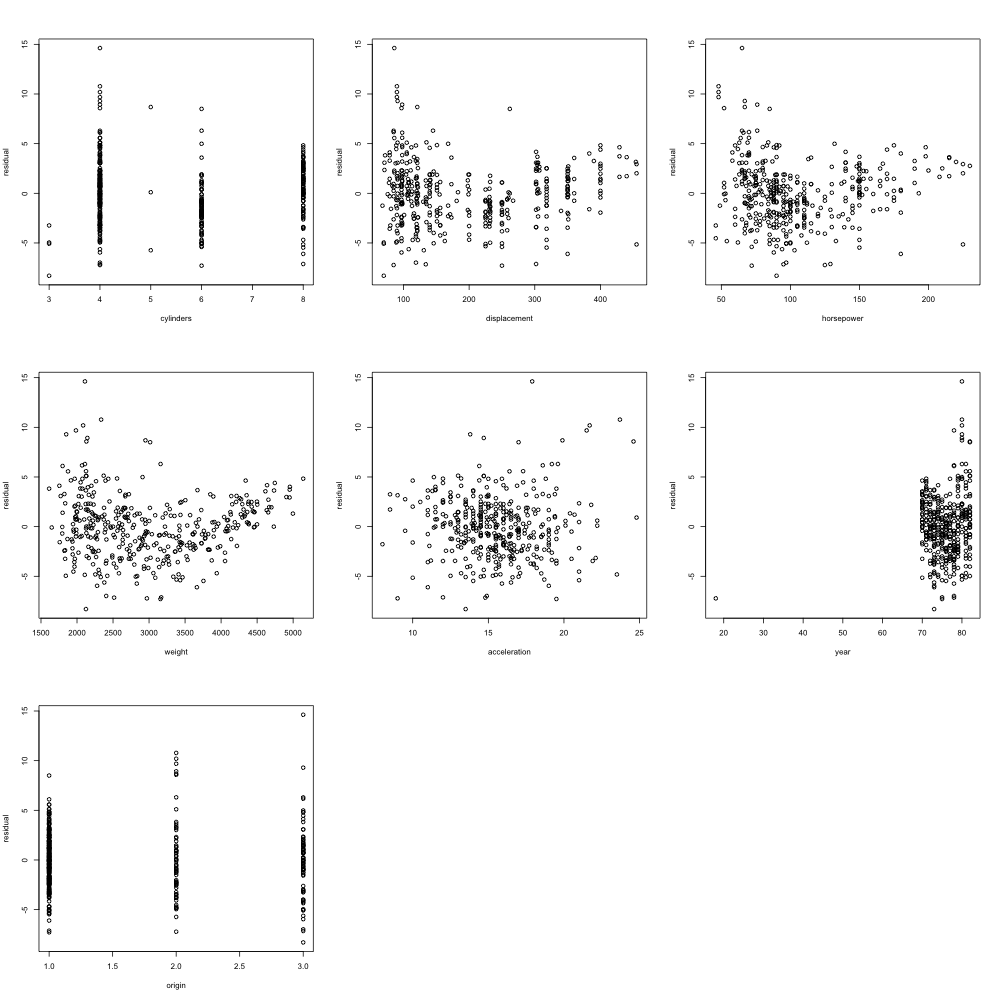
\includegraphics[scale=0.13]{1_res_vs_value}
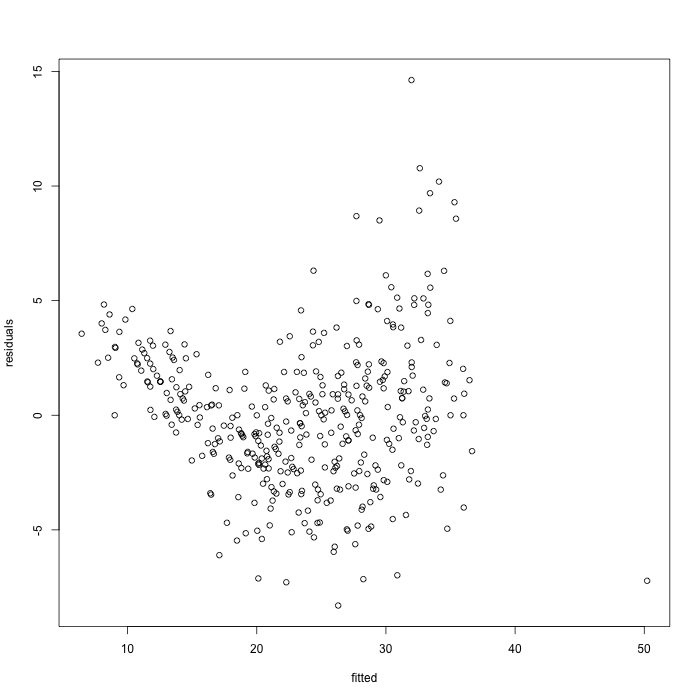
\includegraphics[scale=0.2]{1_res_vs_fitted}
\end{center}
\begin{center}
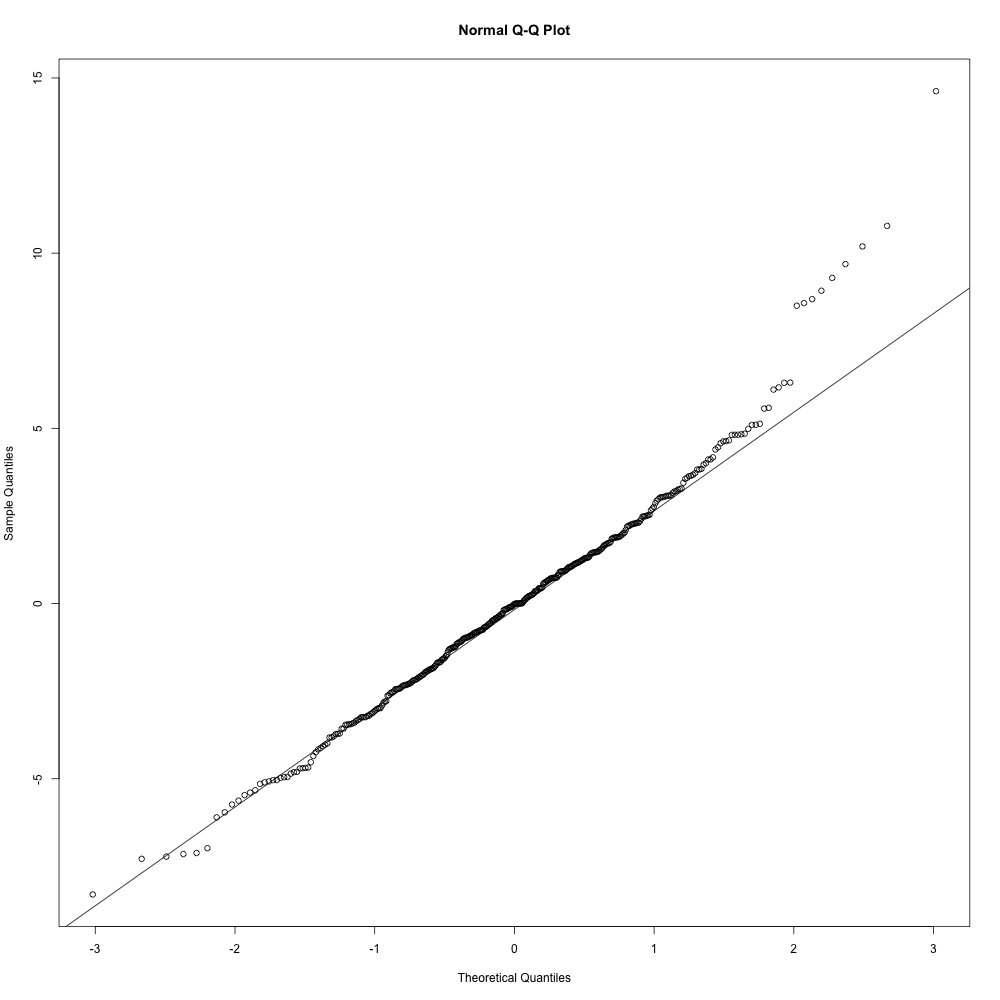
\includegraphics[scale=0.13]{1_QQplot}
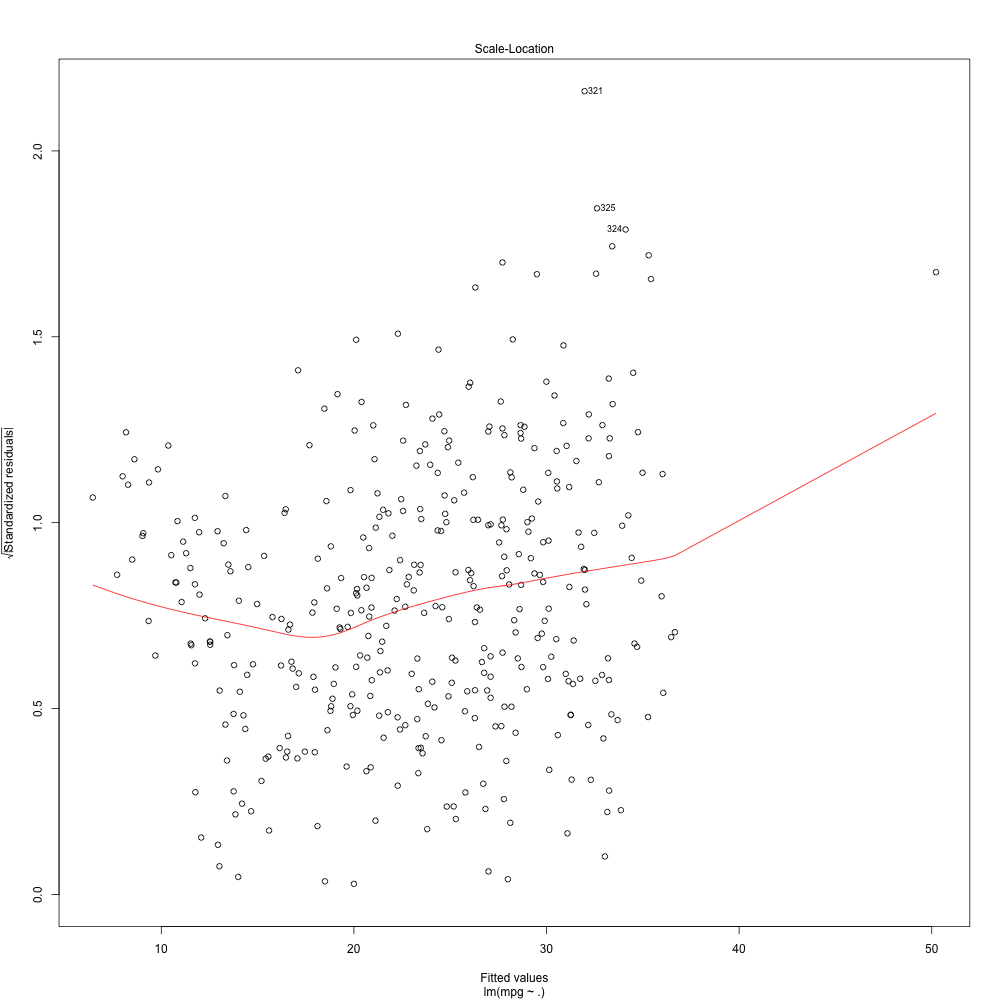
\includegraphics[scale=0.13]{1_Variance}
\end{center}
From the residual vs fitted (top right), the plot show a none linear trends this implies a transformation is needed to make the responds variable(mpg) to be linear.\\
The top right graph which is residual vs fitted we can observe a none-horizontal line across zero. Therefore this may also implies that a stabilizing variance transformation of the mpg is needed.\\
The multiple plots(top left) suggest some of the variable used is not linear. Specifically this suggest displacement, horsepower and weight are not linear. There could also be more.\\
The Q-Q plots(bottom left) seems mostly fine apart from the upper quartile where values diviate from the line drastically. This may pose a problem later on.



\subsection{Reciprocal of Explainatory Variable Models}
The variables displacement, horsepower and weight are assign the reciprocal of it's value. If the model is now fitted around the data the plot obtain to check the assumption of model is:
\begin{center}
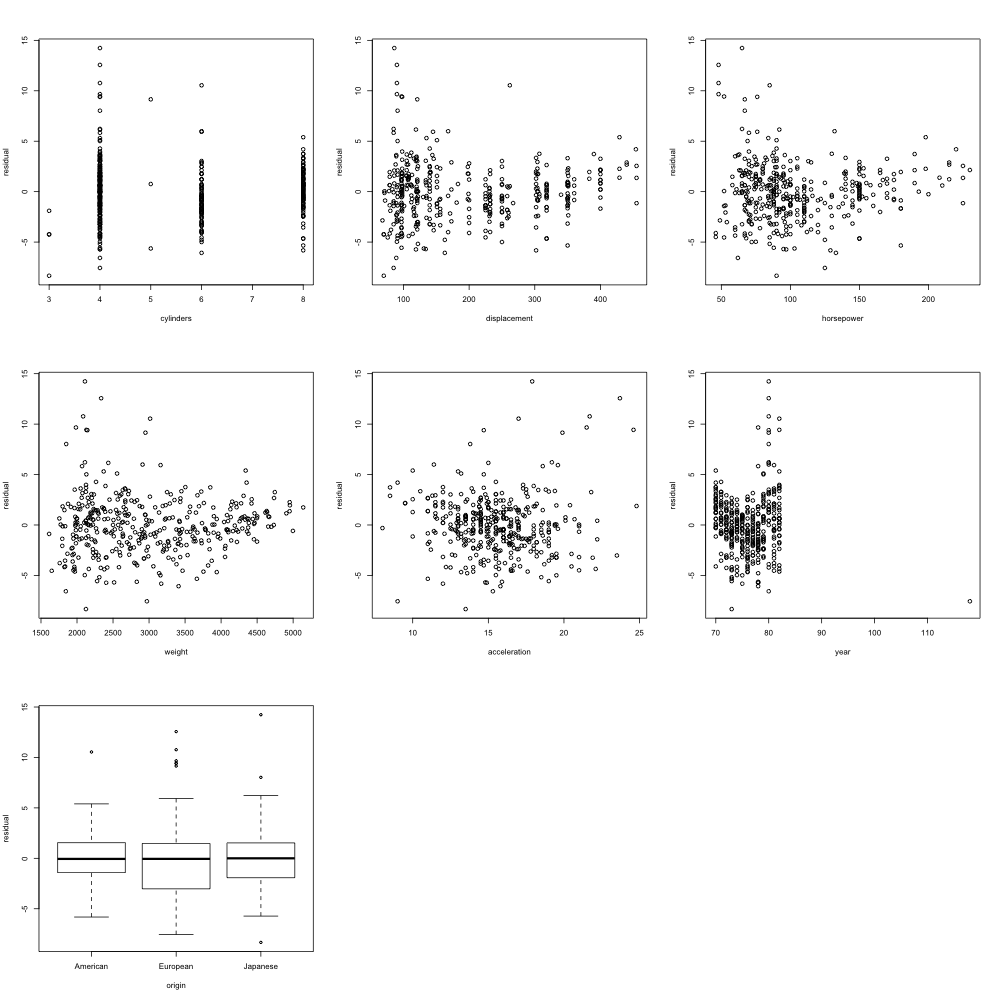
\includegraphics[scale=0.13]{2_res_vs_value}
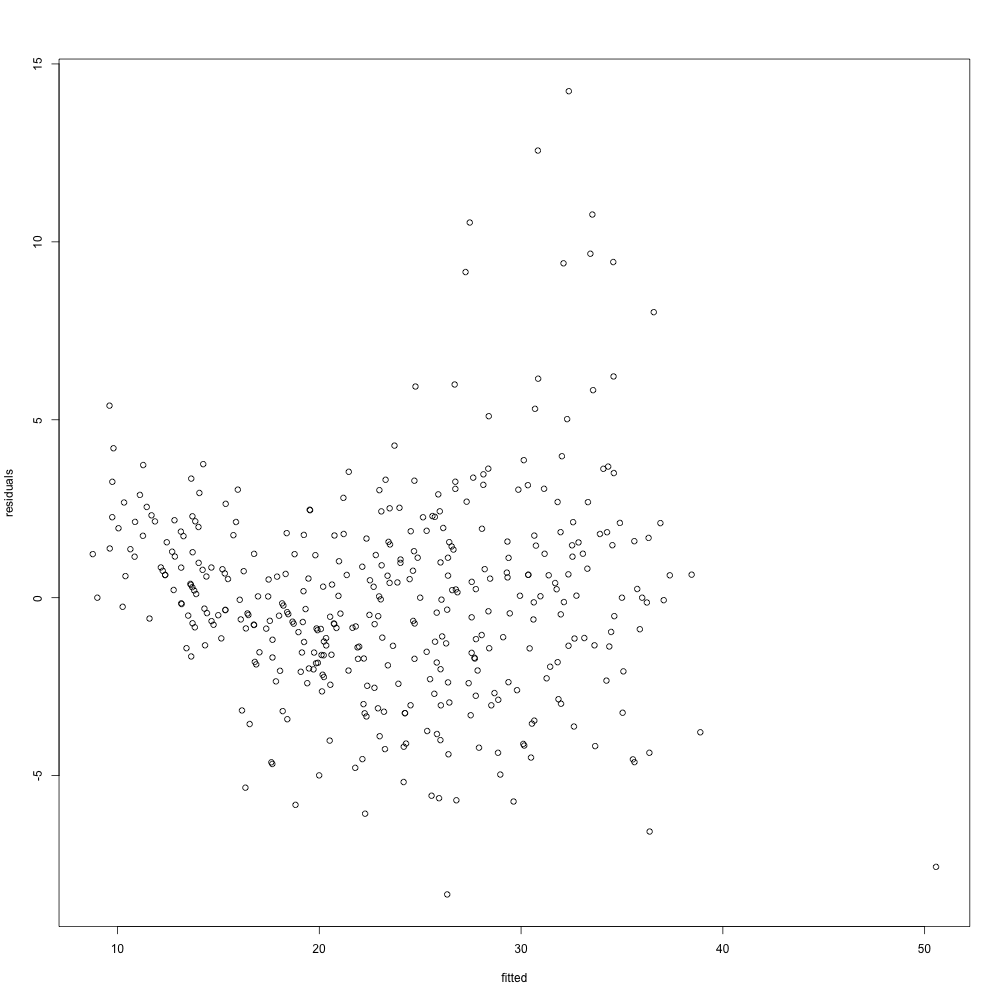
\includegraphics[scale=0.13]{2_res_vs_fitted}
\end{center}
\begin{center}
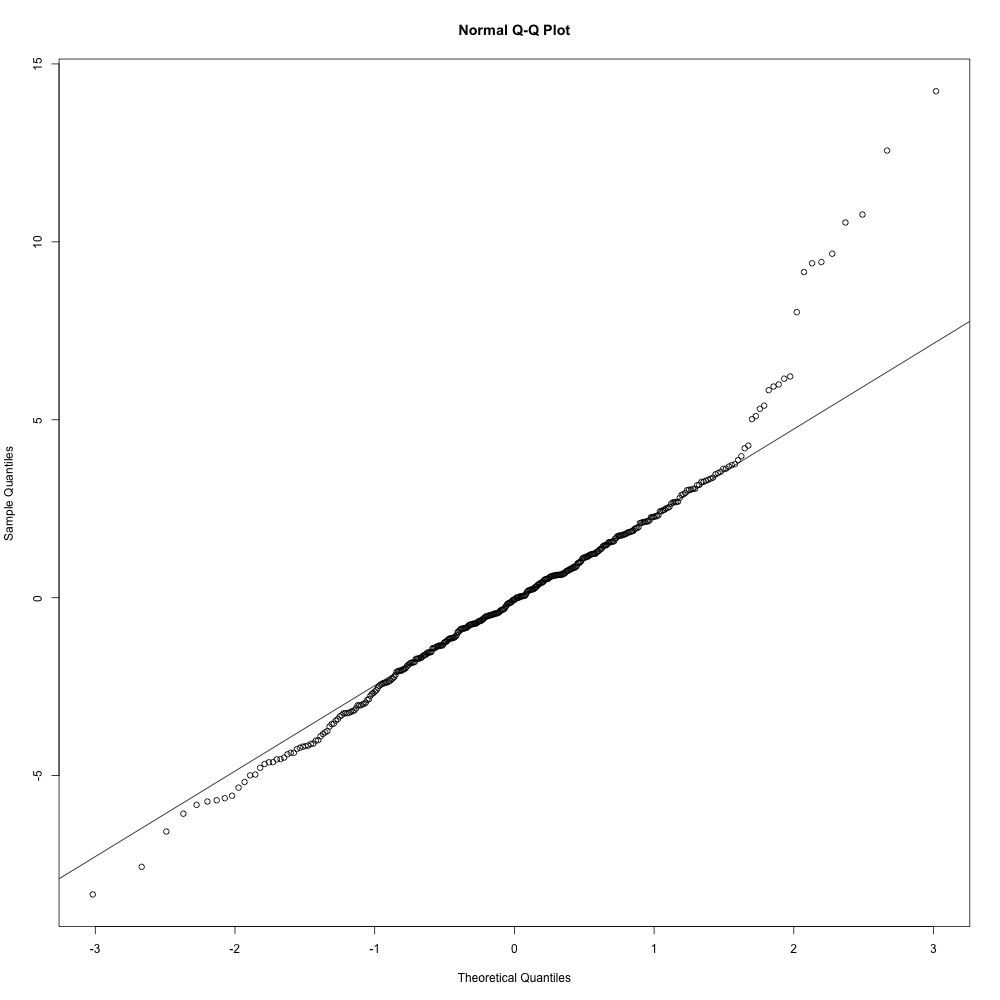
\includegraphics[scale=0.13]{2_QQplot}
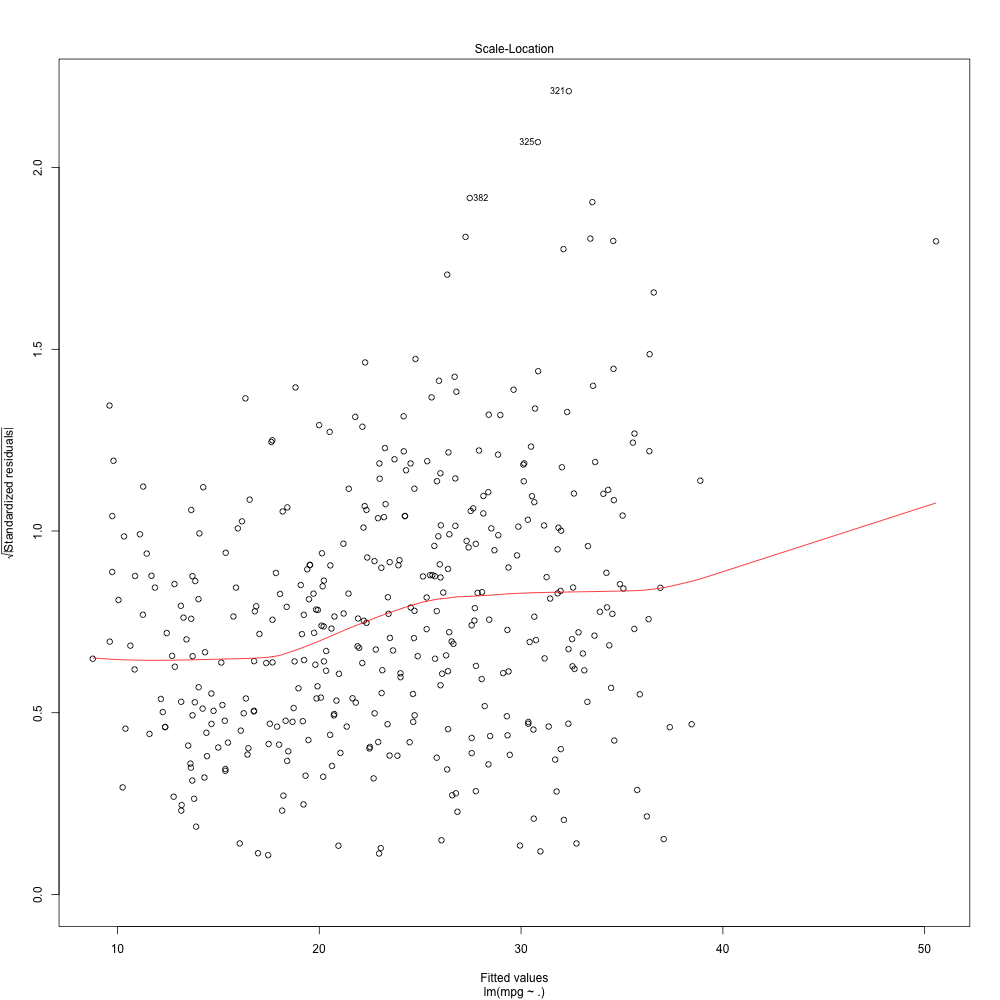
\includegraphics[scale=0.13]{2_Variance}
\end{center}
The diagnostics plots tells us the transformation of the reciprocal of the variable stated above doesn't change the linearity of the model or improve the homoscedacity(bottom right plot) and it's made the normality of the model even worse (bottom right). Therefore we don't use this transformation.\\

\subsection{Square Root Model}
consider a square root transformation of the model where our responds is the square root then:
\begin{center}
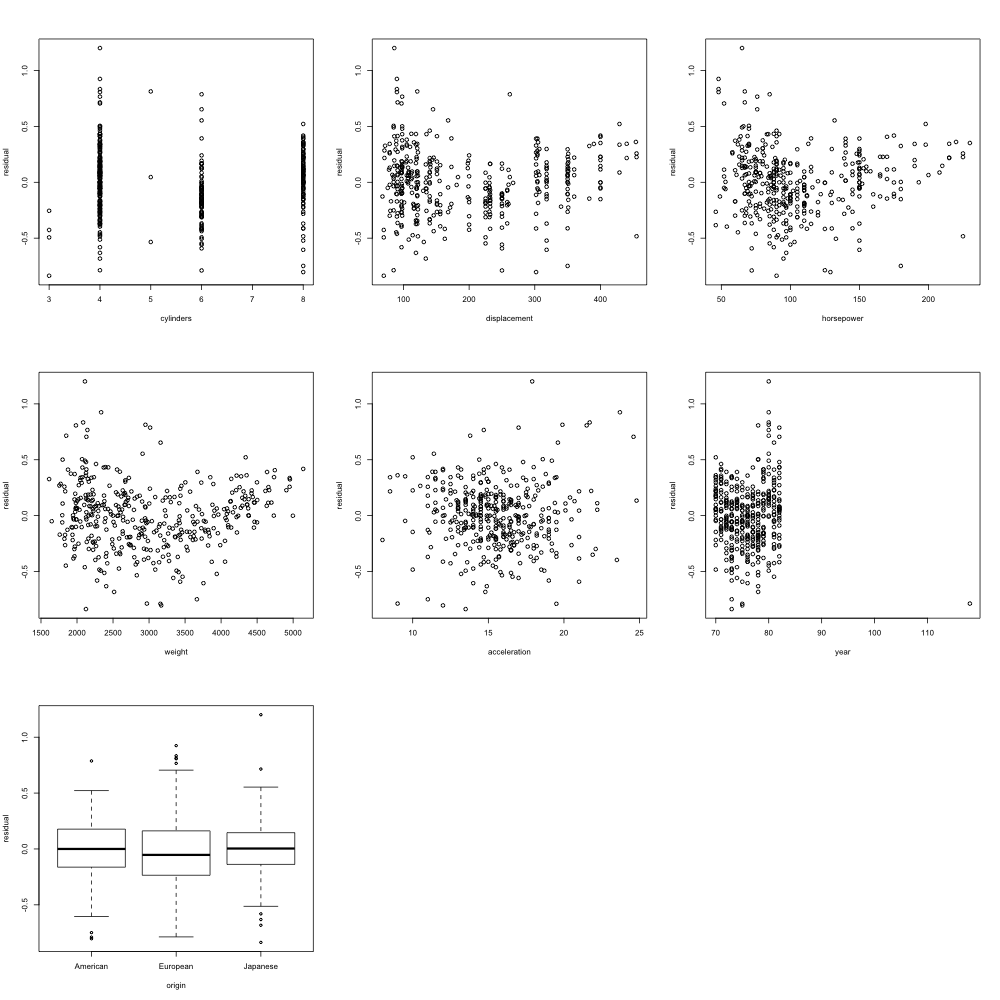
\includegraphics[scale=0.13]{sqrt_res_vs_value}
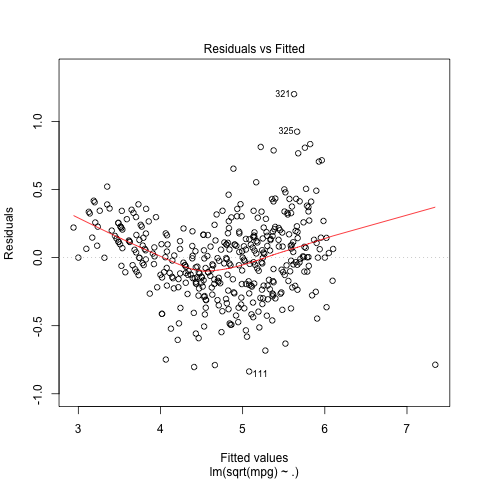
\includegraphics[scale=0.3]{sqrt_res_vs_fitted}
\end{center}
\begin{center}
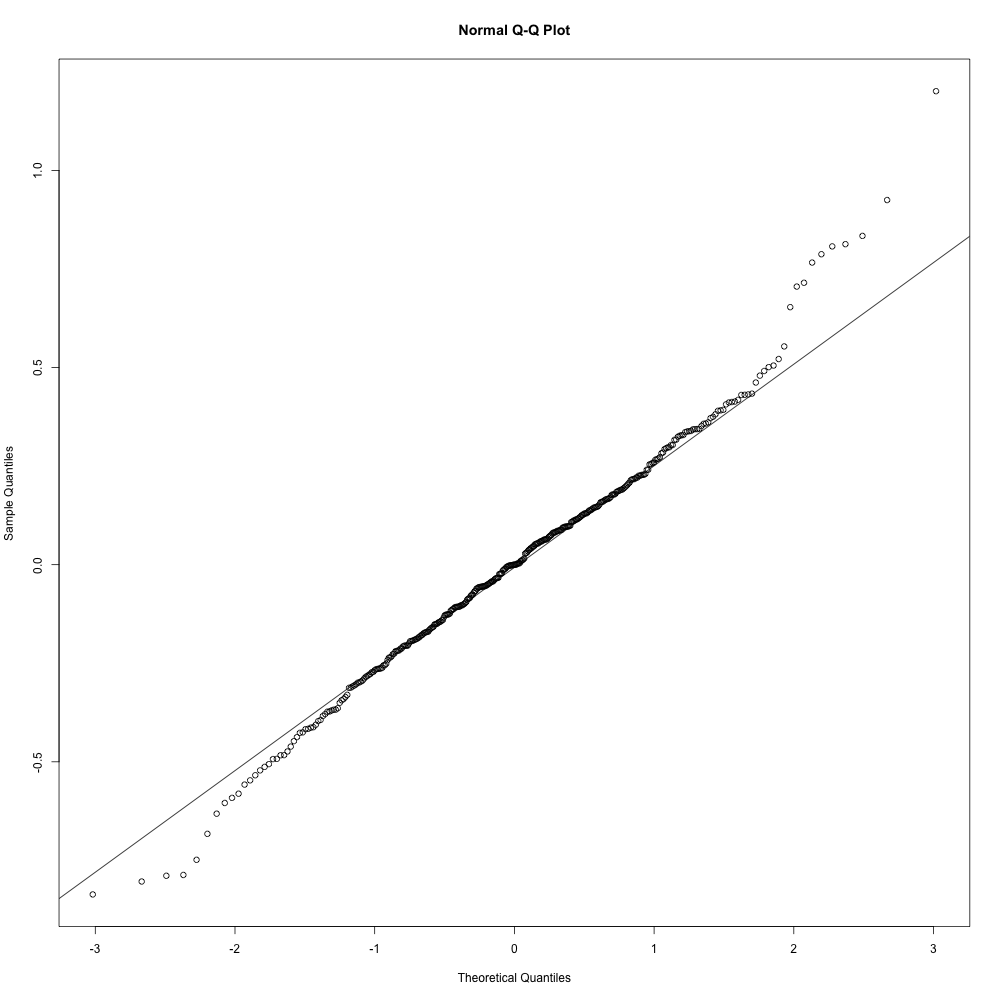
\includegraphics[scale=0.13]{sqrt_QQplot}
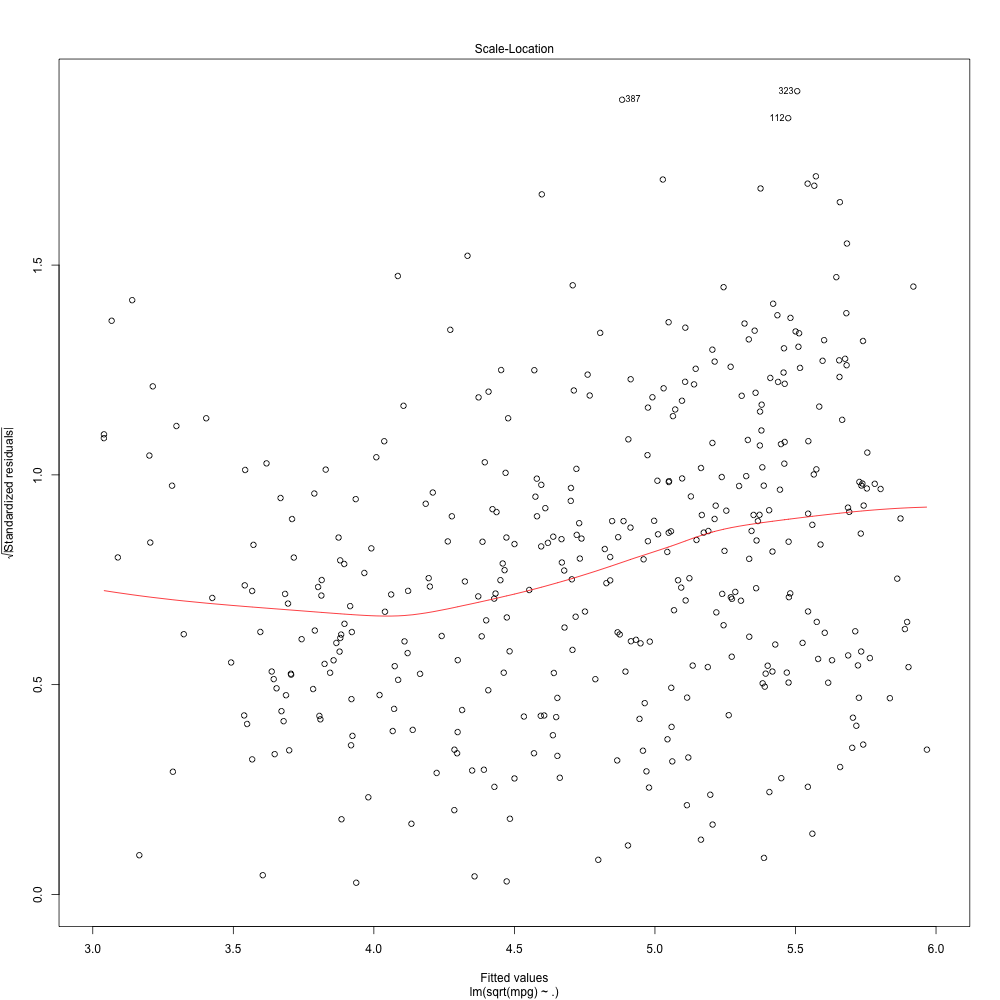
\includegraphics[scale=0.13]{sqrt_Variance}
\end{center}

\subsection{Logarithmic Transformation}
The model in this have been fitted such that it's the logarithmic of the responds variable. The diagnostic plots shows:
\begin{center}
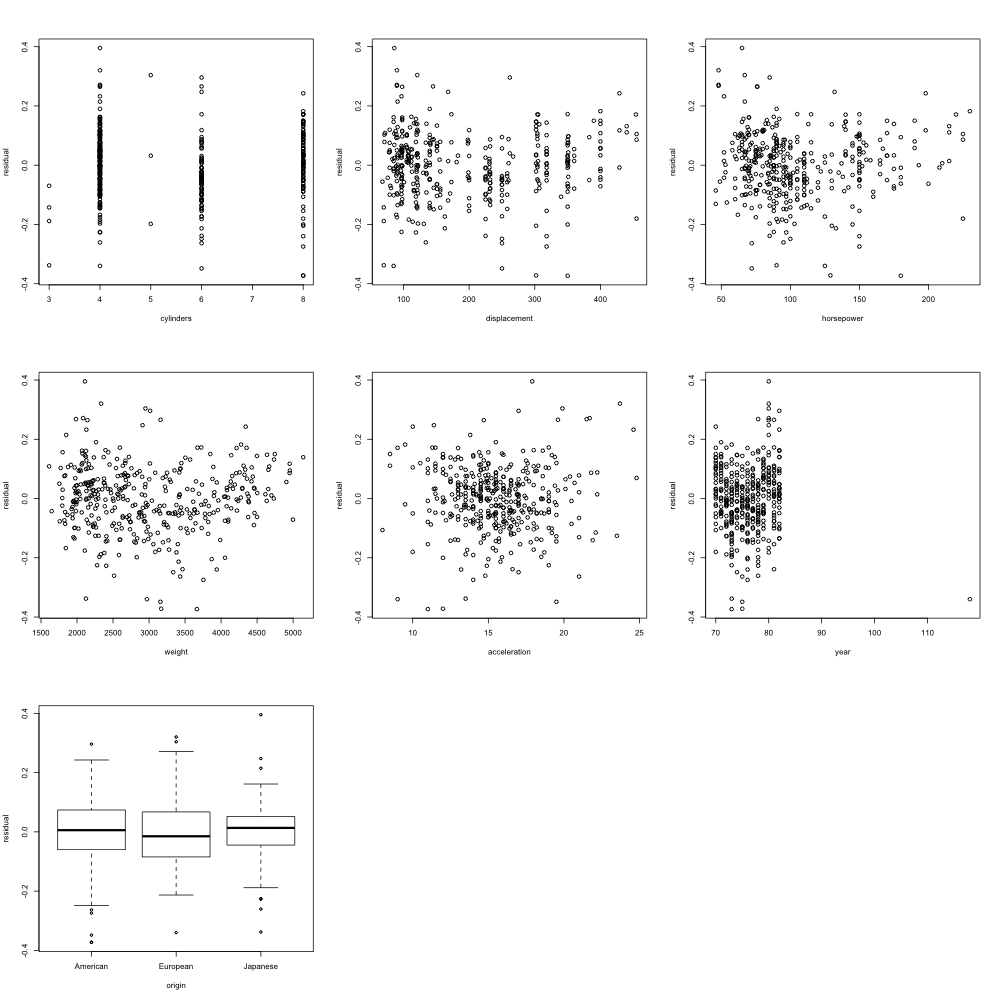
\includegraphics[scale=0.13]{3_res_vs_value}
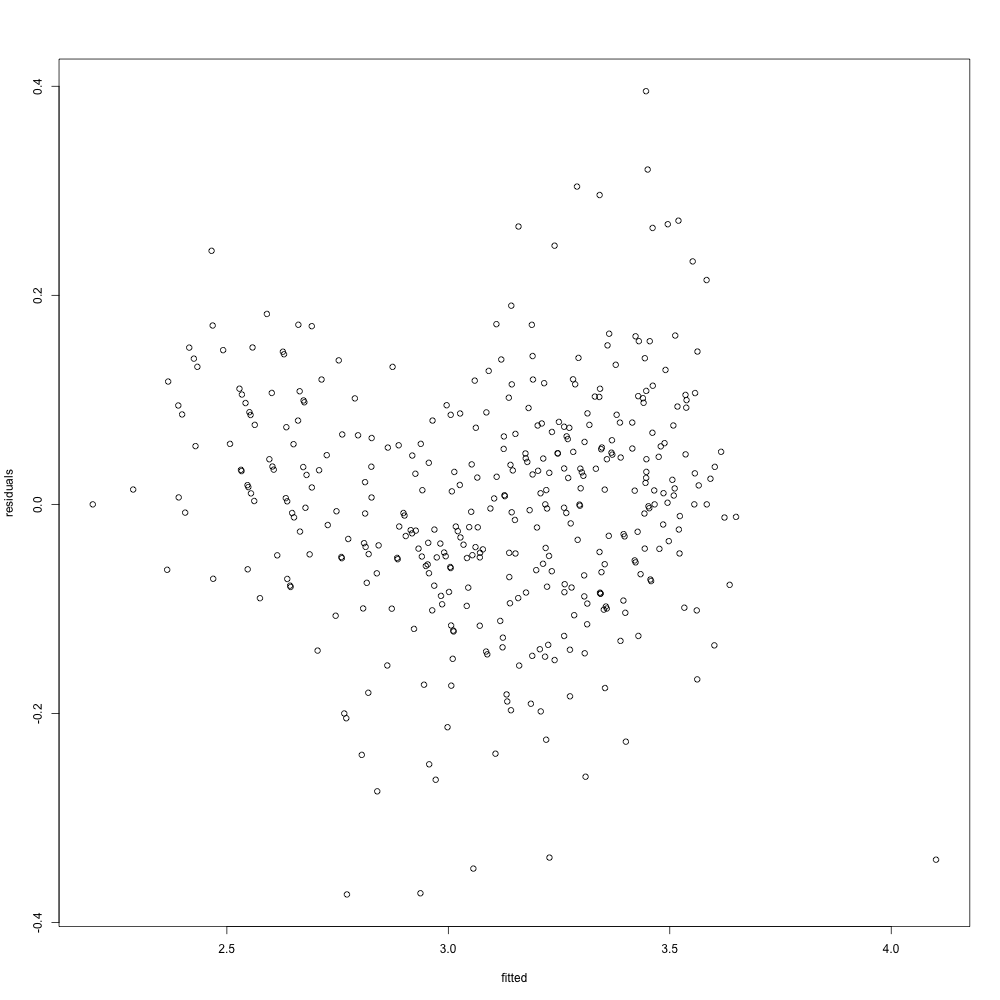
\includegraphics[scale=0.13]{3_res_vs_fitted}
\end{center}
\begin{center}
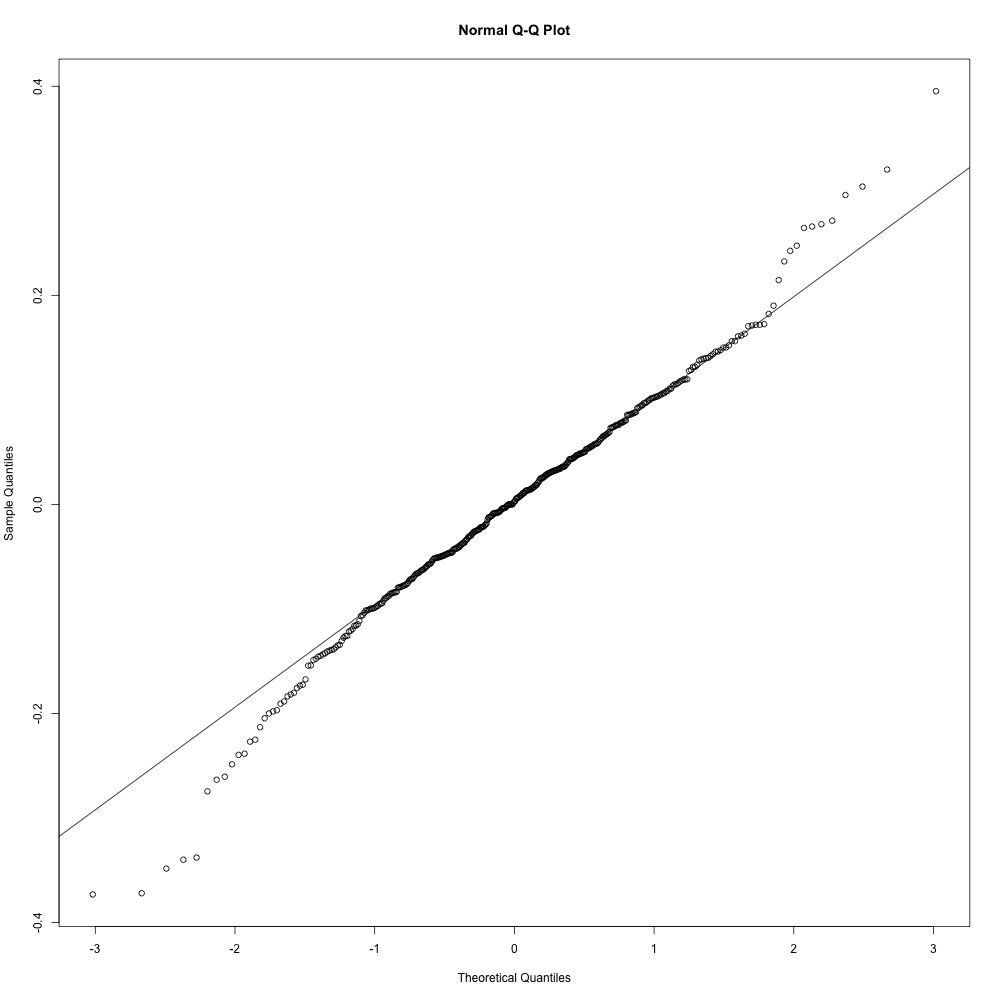
\includegraphics[scale=0.13]{3_QQplot}
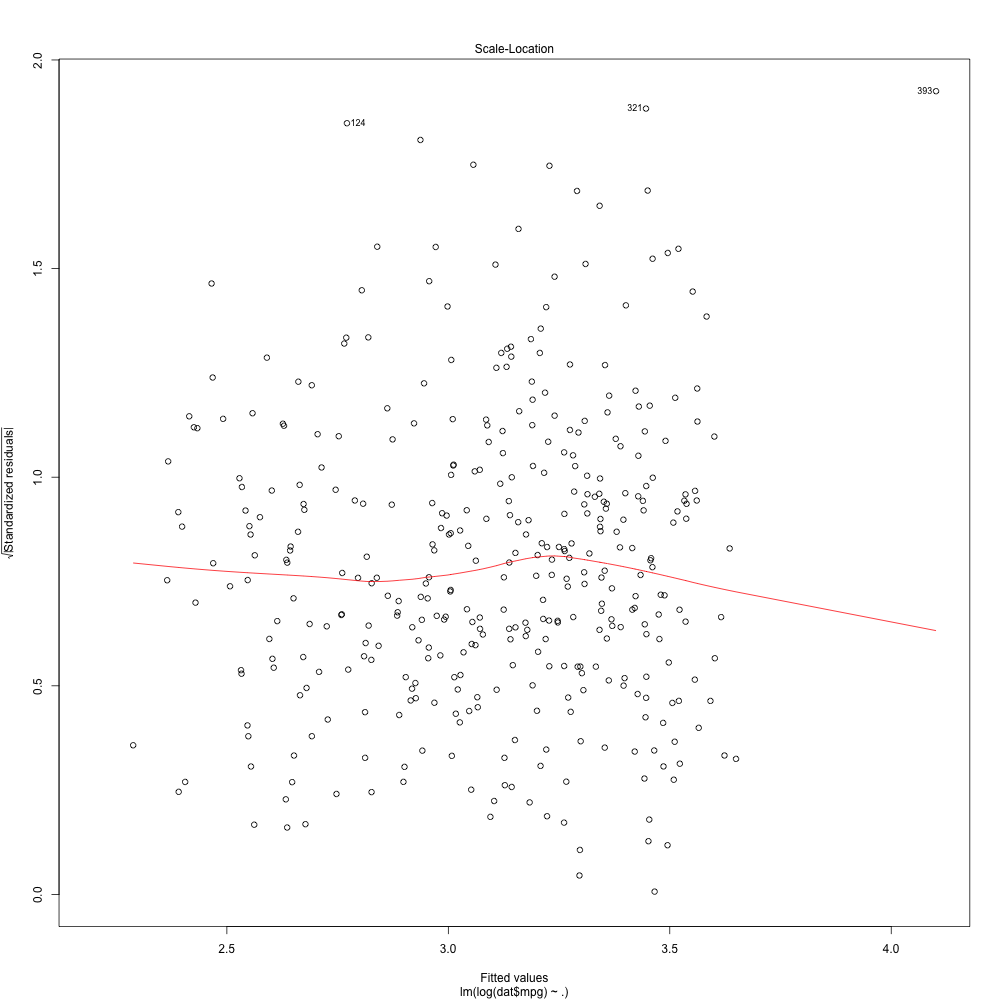
\includegraphics[scale=0.13]{3_Variance}
\end{center}
This is a relatively good transformation. The residual vs explainatory variable(top left) tells us the model now is more linear than it was before.


\subsection{Reciprocal Transformation}
The model in this have been fitted such that it's the reciprocal of the responds variable. The diagnostic plots shows:
\begin{center}
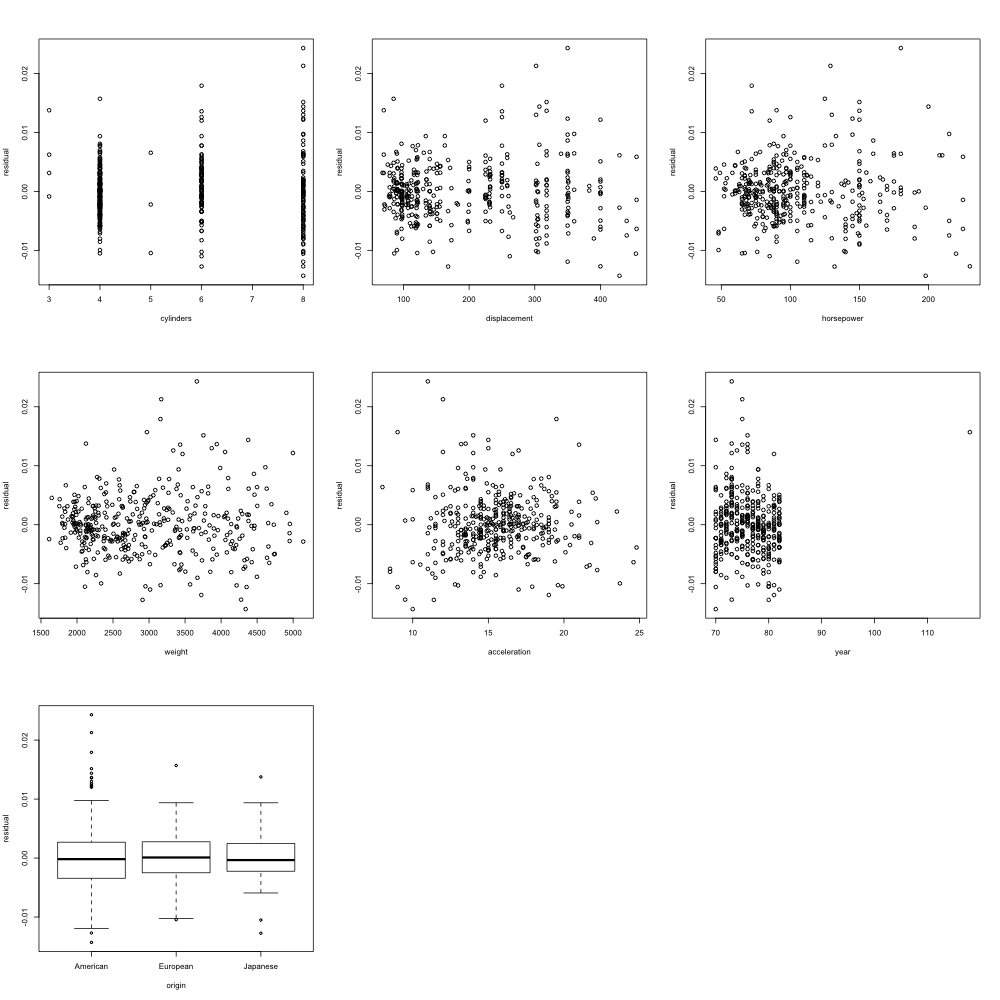
\includegraphics[scale=0.13]{4_res_vs_value}
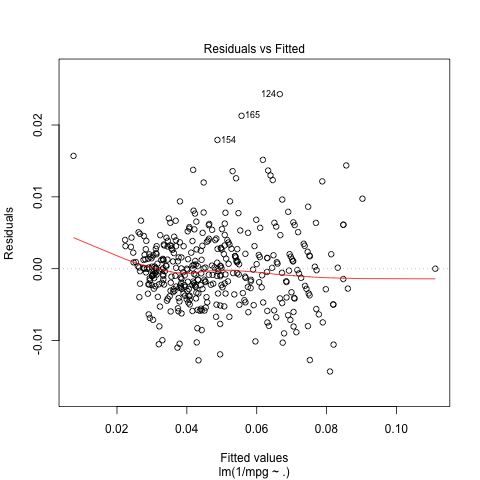
\includegraphics[scale=0.3]{4_res_vs_fitted}
\end{center}
\begin{center}
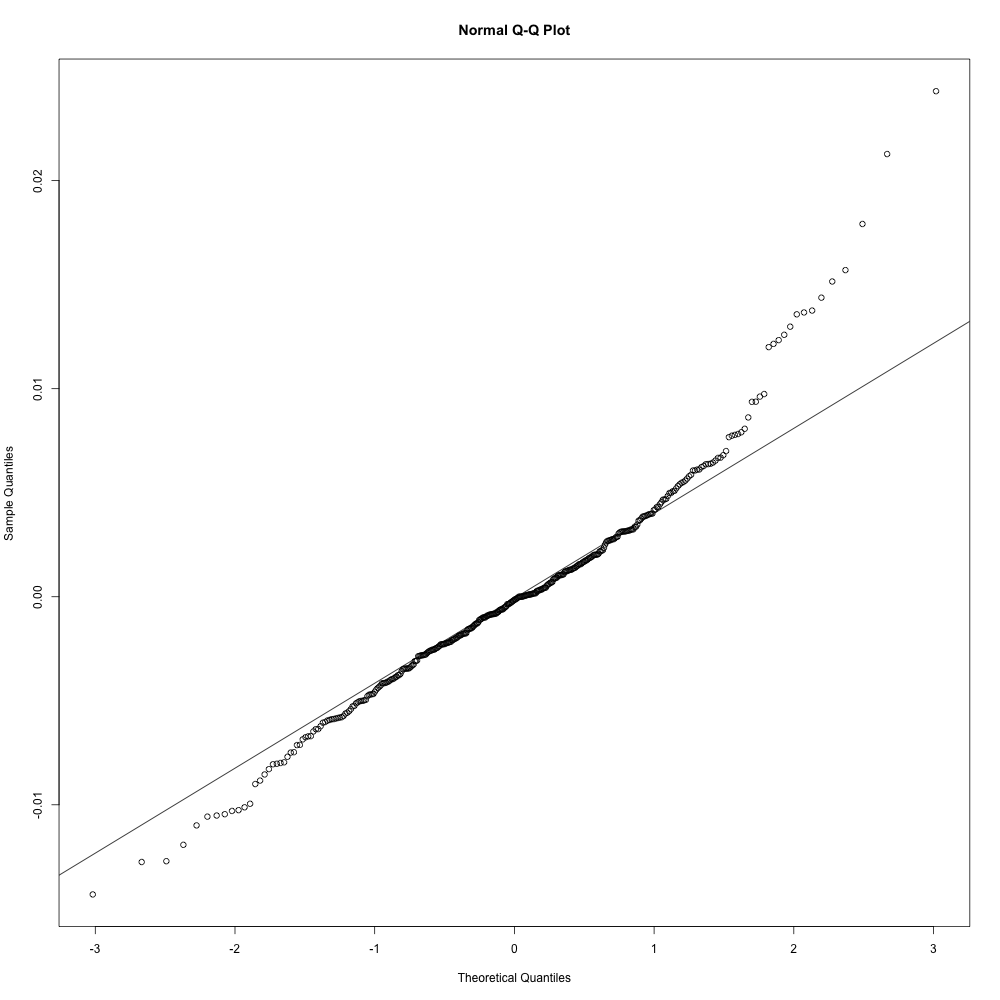
\includegraphics[scale=0.13]{4_QQplot}
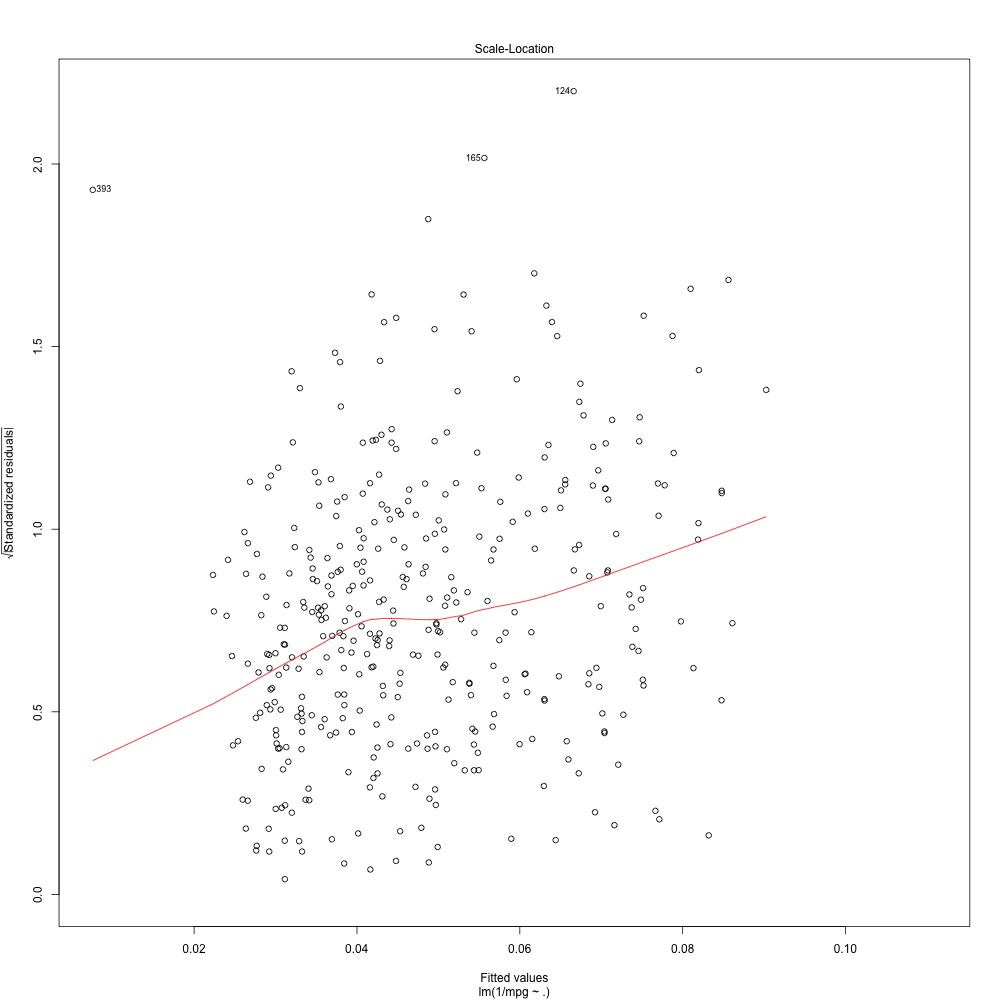
\includegraphics[scale=0.13]{4_Variance}
\end{center}
This model seems to be good for linearity of the model as shown by the explainatory variable(top left) to be more spread out and doesn't have a funnel shape as previous plots. Similarly the same can be said for the residual vs fitted plot. The problem is that this model have made the homoscedacity worse and normality of this model is slightly worse than our original model.

\subsection{Log-Reciprocal model}
This model we perform a transformation of mpg to reciprocal of that then transform it again into a logarithmics reciprocal of the mpg.
\begin{center}
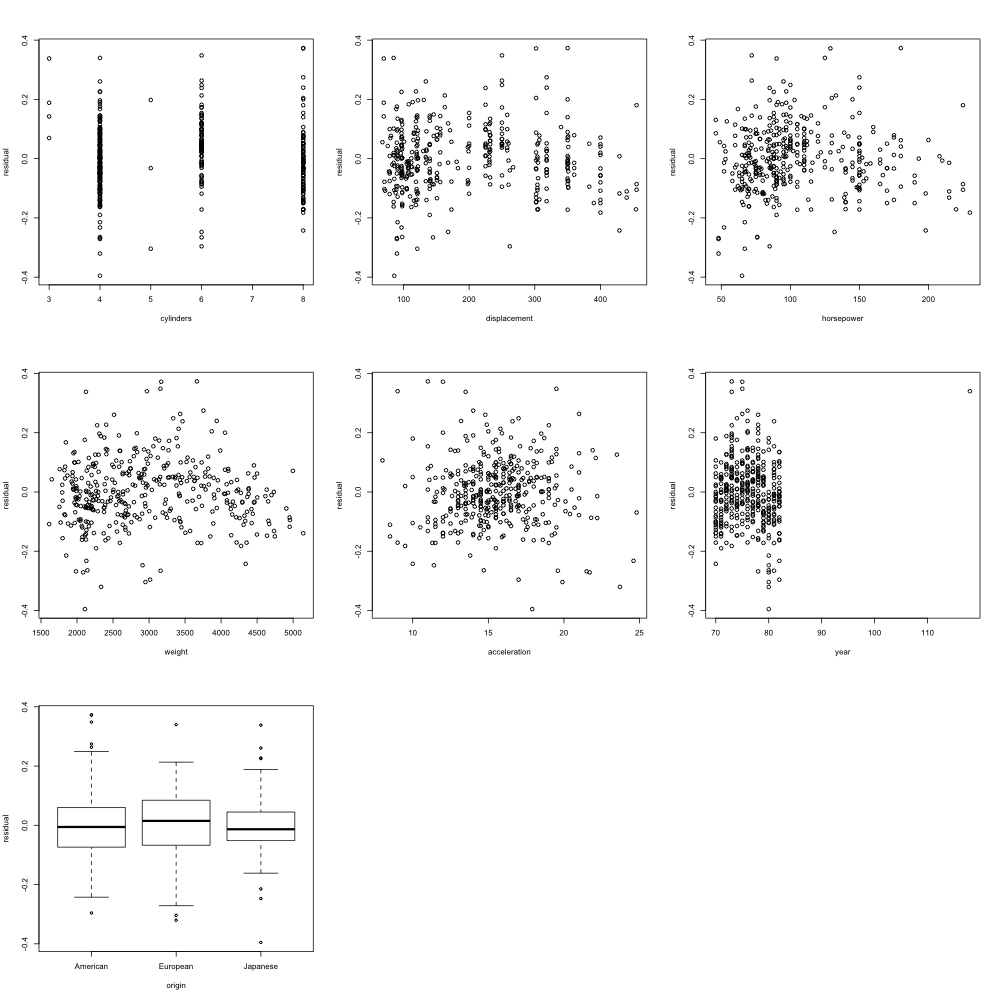
\includegraphics[scale=0.13]{5_res_vs_value}
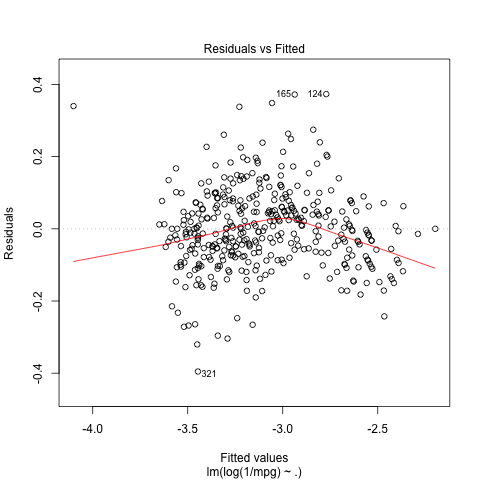
\includegraphics[scale=0.3]{5_res_vs_fitted}
\end{center}
\begin{center}
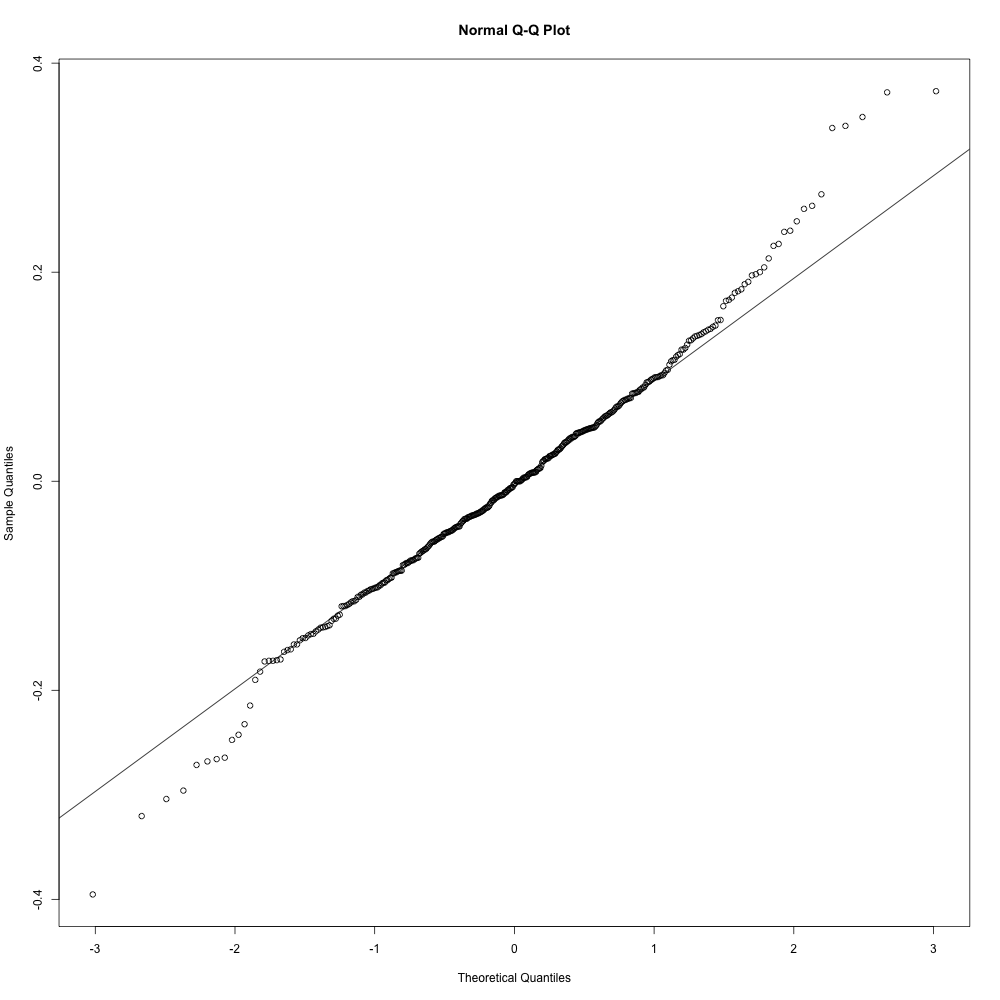
\includegraphics[scale=0.13]{5_QQplot}
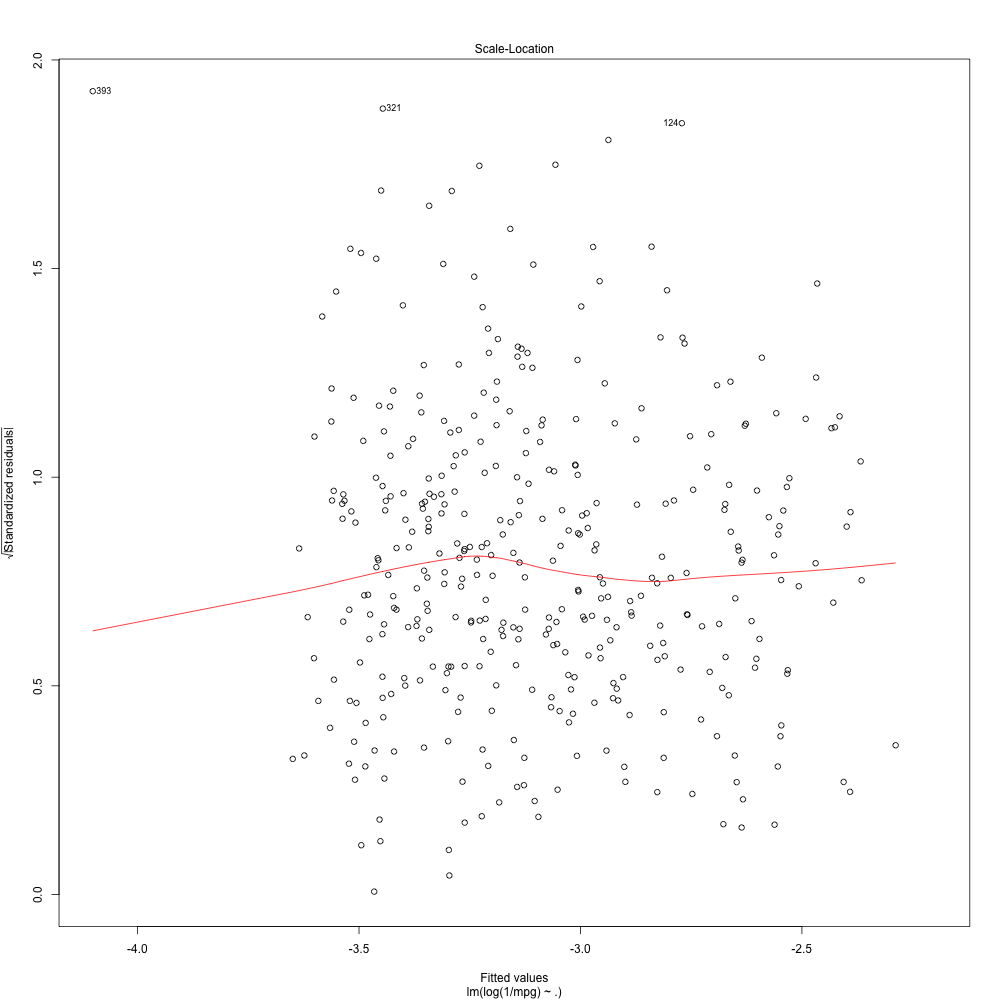
\includegraphics[scale=0.13]{5_Variance}
\end{center}
From this we can observe that the variance is more stablized, from bottom right plot, from the logarithmic tranformation compared to the reciprocal model. The linearity of the model (top right plot) is roughly the same of the reciprocal model, it's not a straight line but it fairs better than the square root transformation or the base model. The normality has improved from the reciprocal model (q-q plot, bottom left). Therefore this model is a good model compared to all the previous model.

\subsection{Box-Cox Transformation}
Since our responds (mpg) is possitive then the Box-Cox transformation is appropriet.

\subsection{Ridge's Regression}

\section{Variables Selection for Models}
In this section we may split the table (observation) into two table. One table is used to fit our model to the data while the other is used to judge how well the model predict given the parameters that model haven't seem before.


\section{Influential Values (Outliers)}
Using residual vs leverage and Cook's distance to check outlier of the data. This may show values in the data which influence our model. Should any be found we may need to remove that observation from our model. 


\newpage
\section{R-Code}
\subsection{Cleaning data}
\begin{lstlisting}
> dat = read.table("http://www1.maths.leeds.ac.uk/~charles/math3714/Auto.csv",
 header = T)
> View(dat)
> summary(dat)
mpg 		cylinders	displacement	 horsepower
Min.   : 9.0	Min.   :3.000	Min.   : 68.0 	Min.   : 46.0
1st Qu.:17.0	1st Qu.:4.000	1st Qu.:105.0	1st Qu.: 75.0
Median :23.0	Median:4.000	Median :151.0	Median : 94.0
Mean   :23.5	Mean   :5.468	Mean   :194.1	Mean   :104.5
3rd Qu.:29.0	3rd Qu.:8.000	3rd Qu.:267.0	3rd Qu.:125.0
Max.   :46.6	Max.   :8.000	Max.   :455.0	Max.   :230.0

weight		acceleration	year		origin
Min.   :1613	Min.   : 8.00	Min.   :18.00	Min.   :1.000
1st Qu.:2226	1st Qu.:13.70	1st Qu.:73.00	1st Qu.:1.000
Median :2807	Median :15.50	Median :76.00	Median :1.000
Mean   :2978	Mean   :15.52	Mean   :75.83	Mean   :1.578
3rd Qu.:3613	3rd Qu.:17.00	3rd Qu.:79.00	3rd Qu.:2.000
Max.   :5140	Max.   :24.80	Max.   :82.00	Max.   :3.000

name
amc matador       :  5
ford pinto        :  5
toyota corolla    :  5
amc gremlin       :  4
amc hornet        :  4
chevrolet chevette:  4
(Other)           :366
\end{lstlisting}
\textbf{Error in Year}
\begin{lstlisting}
> dat$year[dat$name=='vw golf estate S 1.4 TSI'] = 118
> View(dat)
\end{lstlisting}
\textbf{Problems with Names}
\begin{lstlisting}
dat = read.table("http://www1.maths.leeds.ac.uk/~charles/math3714/Auto.csv", header = T, stringsAsFactors = F)
#---Addressing 2nd problem
#In order to achieved this I need to add an extra tag into the 
#dataframe which is "stringAsFactors=F".
#adding a extra entry called make which stands for the maker of the car.
dat$make = dat$name

#changing the string into the first word of the sring.
#Then attaching the first word of the string to make table.
for(string in dat$make){
  substring = strsplit(string, " ")[[1]]
  maker = substring[1]
  print(maker)
  dat$make[dat$make==string]=maker
}

#changing the string into every word apart from the first word.
for(string in dat$name){
  substring = strsplit(string, " ")[[1]]
  print(paste(substring[-1], collapse=' ' ))
  dat$name[dat$name==string]=paste(substring[-1], collapse=' ' )
}
\end{lstlisting}
\textbf{Duplication of Car Makers}
\begin{lstlisting}
>table(dat$make)
amc	audi	bmw	buick	cadillac	capri	chevroelt
27	7	2 	17	2 		1 	1 
chevrolet	chevy	chrysler	datsun 
43		3 	6 		23 
dodge	fiat	ford	hi	honda	maxda	mazda
28 	8	48 	1	13	2	10	
mercedes mercedes-benz	mercury	nissan 
1	 2		11	1 
oldsmobile	opel 	peugeot	plymouth	pontiac	renault
10		4	8	31		16	3
saab	subaru	toyota	toyouta	triumph
4	4	25	1	1 
vokswagen	volkswagen 	volvo	vw 
1		15		6	7 
\end{lstlisting}
\begin{lstlisting}
>dat$make = factor(dat$make)
>dat$origin[dat$origin==1]='American'
>dat$origin[dat$origin==2]='European'
>dat$origin[dat$origin==3]='Japanese'
>dat$origin = factor(dat$origin)
\end{lstlisting}
\textbf{Uniqueness of Name}
\begin{lstlisting}
#---Problem 5
dat$name=NULL
\end{lstlisting}
\textbf{Multicollinearity}
\begin{lstlisting}
> X=as.matrix(cbind(dat$cylinders,dat$displacement,dat$horsepower,
dat$weight,dat$acceleration,dat$year))
> round(diag(solve(t(X)%*%X)),3) 
[1] 0.009 0.000 0.000 0.000 0.001 0.000
> v=eigen(t(X)%*%X)
> round(v$values,1)
[1] 3791200361.7    1365742.4     130921.6      68541.8       1553.3        111.5
> round(max(v$values)/v$values,0)
[1]        1     2776    28958    55312  2440751 34013500
> round(v$vectors,1)
     [,1] [,2] [,3] [,4] [,5] [,6]
[1,]  0.0  0.0  0.0  0.0  0.0    1
[2,] -0.1 -0.9  0.0 -0.3  0.0    0
[3,]  0.0 -0.2  0.9  0.4 -0.1    0
[4,] -1.0  0.1  0.0  0.0  0.0    0
[5,]  0.0  0.1  0.0 -0.2 -1.0    0
[6,]  0.0  0.3  0.4 -0.8  0.2    0
> S=svd(X)
> S$d
[1] 61572.72417  1168.64981   361.83087   261.80486    39.41183    10.55754
> max(S$d)/S$d
[1]    1.00000   52.68706  170.16990  235.18557 1562.29040 5832.10936
\end{lstlisting}
\subsection{Models}
\textbf{First Model}
\begin{lstlisting}
#MODELS----------------------------------------------------------------------
#First function with no transformation or interactions
base_model = function(dat){
  return(lm(mpg~.,data = dat))
}

#square root model
sqrt_model = function(dat){
  return(lm(sqrt(mpg)~., data=dat))
}

#logarithmic model
log_model = function(dat){
  return(lm(log(mpg)~., data = dat))
}

recip_y = function(dat){
  return(lm(1/mpg ~., data = dat))
}

#reciprocal of certain variable
model2 = function(dat){
  dattemp=dat
  dattemp$displacement=1/dattemp$displacement
  dattemp$weight=1/dattemp$weight
  return(lm(mpg~.,data = dattemp))
}
\end{lstlisting}
\subsection{Diagnostics}
\begin{lstlisting}
#DIAGNOSTICS----------------------------------------------------------------
Res_VS_value=function(model_no,model,dat){
  #saving plot
  png(paste(model_no,"res_vs_value.png",sep = "_"))
  #Residual vs variables not including the make of the car
  no_variable = 7
  res = model$residuals
  dattemp=cbind.data.frame(dat$cylinders,dat$displacement,
  dat$horsepower,dat$weight,dat$acceleration,dat$year,dat$origin)
  colnames(dattemp)=c("cylinders","displacement","horsepower",
  "weight","acceleration","year","origin")
  par(mfrow=c(3,3))
  for(i in 1:no_variable){
    print(names(dattemp)[i])
    plot(dattemp[,i],res,ylab = "residual",xlab = toString(names(dattemp)[i]))
  }
  dev.off()
  
  #plotting the plot
  for(i in 1:no_variable){
    print(names(dattemp)[i])
    plot(dattemp[,i],res,ylab = "residual",xlab = toString(names(dattemp)[i]))
  }
}

Res_VS_fit=function(model_no,model){
  #save the plot
  png(paste(model_no,"res_vs_fitted.png",sep = "_"))
  plot(model,1)
  dev.off()
  
  #plot the plots
  plot(preds,res,xlab = "fitted",ylab = "residuals")
  
}

Normal=function(model_no,model){
  #saving plot
  png(paste(model_no,"QQplot.png",sep = "_"),width = 1000,height = 1000)
  res = model$residuals
  qqnorm(res)
  qqline(res)
  dev.off()
  
  #plot the plot
  qqnorm(res)
  qqline(res)
}

HomoSce=function(model_no,model){
  #plotting
  plot(model,3)
  
  #saving plot
  png(paste(model_no,"Variance.png",sep = "_"),width = 1000, height = 1000)
  plot(model,3)
  dev.off()
}

check_assumption=function(model_no,model,dat){
  HomoSce(model_no,model)
  Normal(model_no,model)
  Res_VS_value(model_no,model, dat)
  Res_VS_fit(model_no,model)
}
\end{lstlisting}
\subsection{Diagnostics of the Model}
\begin{lstlisting}
#Diagnostics-of-Model--------------------------------------------------------
#Running these codes will force save the plots onto the disk.
base = base_model(dat)
square_root = sqrt_model(dat)
Log_model = log_model(dat)
rec_y = recip_y(dat)
model1 = model2(dat)
log_recip_model = lm(log(1/mpg)~., data = dat)

check_assumption("base",base,dat)
check_assumption("model1",model1,dat)
check_assumption("sqrt",square_root,dat)
check_assumption("log",log_model,dat)
check_assumption("reciprocal",rec_y,dat)
check_assumption("log_reciprocal",log_recip_model,dat)
\end{lstlisting}
\end{document}
